% $Id: evaluation.tex 1784 2012-04-27 23:29:31Z nicolas.cardozo $
% !TEX root = main.tex

\chapter{Evaluation}
\label{cha:evaluation}

To evaluate and validate this tool as a framework for the quality development 
of \ac{RL} programs, an initial empirical test is proposed with different scenarios 
that may arise in the development of \ac{RL} programs. These scenarios range from 
the creation of an \ac{RL} program from scratch to the process of optimizing 
learning parameters, aiming to determine the specific values to start with 
to achieve the most optimal convergence for the program.

Subsequently, an evaluation of the tool is proposed with a group of students 
from the \ac{RL} course at the University of the Andes, in order to obtain 
feedback on the utility of the tool and potential improvements that can be made, 
and the utility in general of back in time debuggers for debugging \ac{RL} programs.

Let's dive into the three exercises proposed for the evaluation of the tool. 

\section{Exercise 1: GridWorld}

The gridworld environment consists of a $n\times n$ ($10\times 10$ in our example) rectangular 
board/grid, in which each tile $(i,j)$ represents a specific state of the board. Tiles in the board may be 
walls, which agents cannot cross. Additionally, there are special exit 
tiles that give a positive or negative reward to agents, as shown in \fref{fig:gridworld}. All tile types 
are unknown to the agent that moves from a given starting point in the board, searching for the goal 
state (\ie exit states with positive reward of 1). The agent moves from state to state, avoiding 
obstacles and incorrect exit states (which give a reward of $-1$ when used to exit). The gridworld 
dataset contains 20 implementation instances. 

\begin{figure}[h]
  \centering
  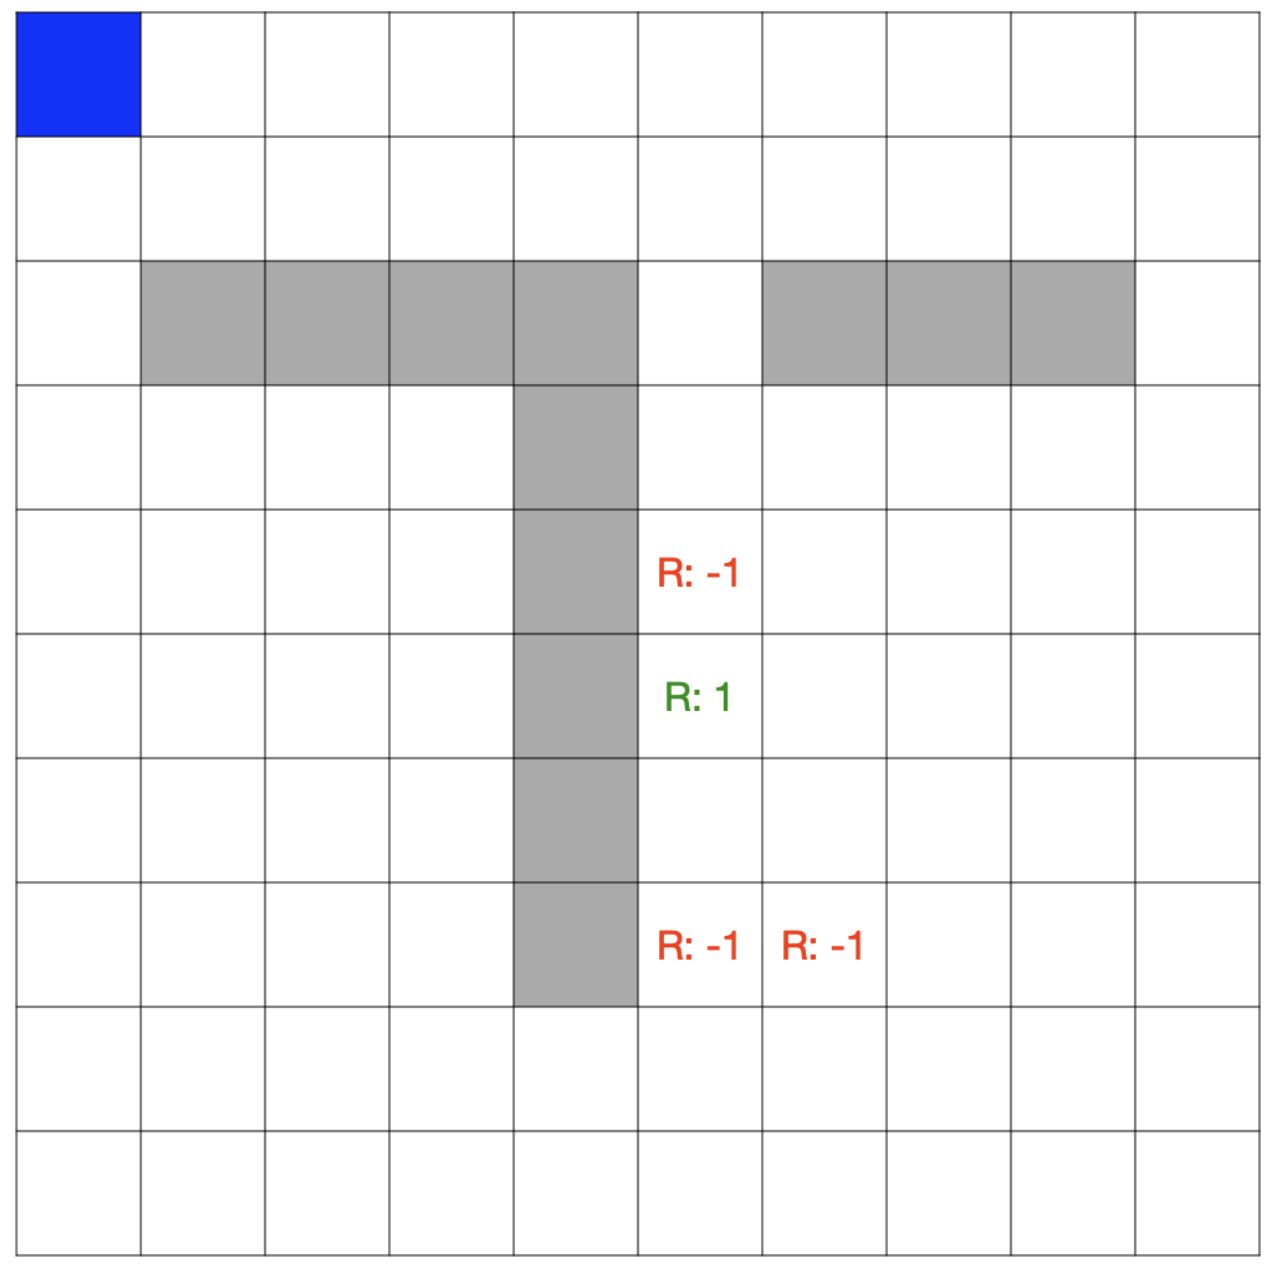
\includegraphics[width=0.5\columnwidth]{figures/gridworld.png}
  \caption{10x10 gridworld environment example}
  \label{fig:gridworld}
\end{figure}

Now in this example is to play with the probabilities in which the action is taken, changing 
the epsilon value, so the student needs to realized that they have to change the value of 
alpha, the idea then is to use the debugger in order to understand this wrong behavior.

\section{Exercise 2: Rooms}

The four rooms maze environment consists of a $13\times 13$ board/grid divided in 4 sections 
(\ie rooms), with walls between them, and a door opening to go from one room to another, as shown 
in \fref{fig:rooms}. The agent's objective in this environment is to exit through the upper-left room 
(the green square) in the fewest possible steps. Reaching the exit state gives a reward of 1, and no 
other action give a reward to the agent.
In each episode the agent starts from any valid position in the grid, \eg the yellow square in the 
bottom-right room in the figure. The rooms dataset contains 23 implementation instances.

\begin{figure}[h]
  \centering
  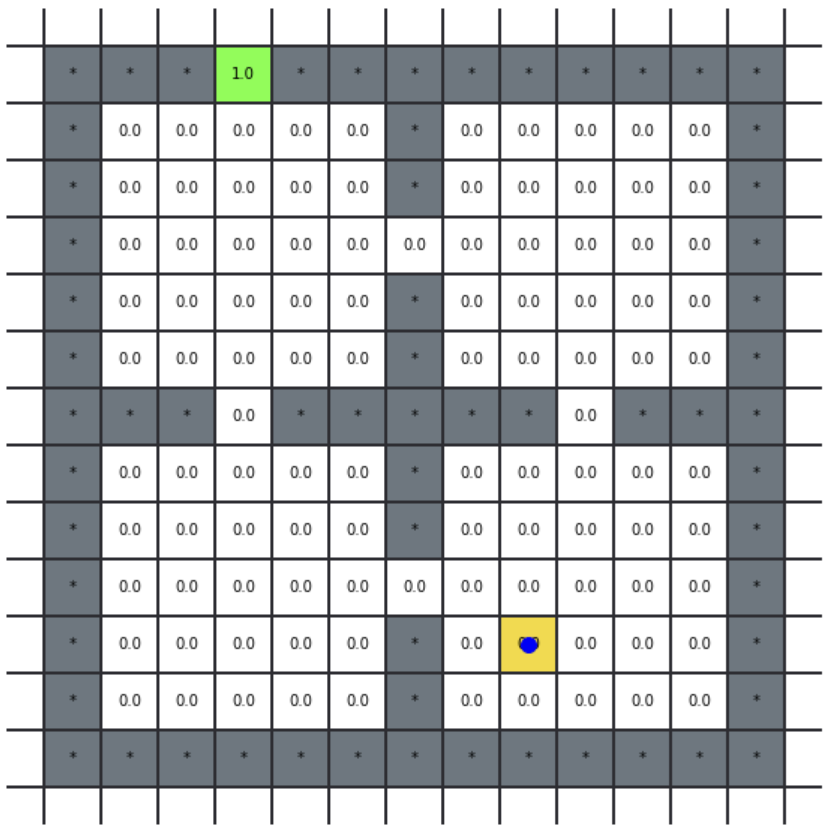
\includegraphics[width=0.5\columnwidth]{figures/rooms.png}
  \caption{Rooms environment example with associated rewards in each state}
  \label{fig:rooms}
\end{figure}

Now in this example the idea is to change the QLearning equation so the original values for 
the learning rate alpha are exchanged like:

Original equation:
$
Q(s, a) \leftarrow (1-\alpha) Q(s, a) + \alpha \left( r + \gamma \max_{a'} Q(s', a') - Q(s, a) \right)
$

Wrong equation to debug:
$
Q(s, a) \leftarrow  \alpha Q(s, a) + (1-\alpha) \left( r + \gamma \max_{a'} Q(s', a') - Q(s, a) \right)
$
So the idea is that the student realizes this issue and solves it using the back in time debugger.

\endinput

